\documentclass[../../main.tex]{subfiles}
\usepackage{pgfplots}
\pgfplotsset{compat=1.18}
\begin{document}
\chapter{Intermediate Blocks, AZee Templates and Pose Correction}
\label{ch:intermediate_blocks_pose_correction}

Creativity in human expression often lies at the intersection of structure and flexibility. In Sign Language, meaning is not just conveyed through individual signs but through the seamless transitions and interactions between them. These transitions, or intermediate blocks, play a crucial role in maintaining the natural flow of communication, ensuring that the message remains clear and expressive.

Generating these intermediate blocks in multi-track representations requires a blend of procedural precision and adaptive techniques. The complexity of Sign Language demands more than linear models; it requires an approach that can reflect the nuances of real-life communication. By integrating the AZee model with multi-track timelines, this chapter explores how we can improve the accuracy and fluidity of synthesized Sign Language.

This chapter focuses on the generation of intermediate blocks within the multi-track representations introduced in chapter~\ref{ch:multi-track}. By utilizing motion templates and carefully interpolating between keyframes, we aim to enhance the naturalness and coherence of Sign Language synthesis.

In this chapter, section~\ref{ch:intermediate_blocks_pose_correction:related_work} discusses the related work on AZee Templates, Motion Curves, and Motion Templates. Section~\ref{ch:intermediate_blocks_pose_correction:intermediate_block_generation} explores the generation of intermediate blocks, while section~\ref{ch:intermediate_blocks_pose_correction:results} presents the results of this process. Finally, section~\ref{ch:intermediate_blocks_pose_correction:conclusion_and_future_work} concludes the chapter and outlines potential future directions for this research.

\section{Intermediate Block Generation}
\label{ch:intermediate_blocks_pose_correction:intermediate_block_generation}

Intermediate blocks are blocks of motion not specified by the AZee model. Building on the concepts of motion curves and templates, intermediate block generation is a process in creating smooth transitions between constrained and pre-animated blocks. Interpolation techniques, such as linear and spline interpolation, can be used to generate intermediate poses or frames that maintain the semantic consistency of the intended sign. Figure ~\ref{fig:info_about_intermediate_example} shows intermediate blocks generated for the AZee rule \emph{info-about(topic,info)}.

\begin{figure}
    \centering 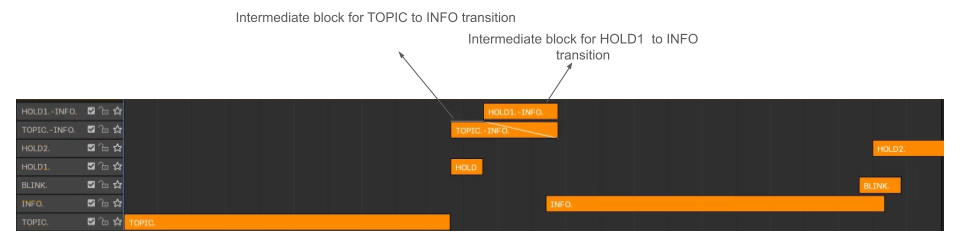
\includegraphics[width = 5in]{chapters/intermediate_blocks/images/info_about_intermediate_example.png}
    \caption{Intermediate Blocks for the AZee rule \emph{info-about(topic,info)}}
    \label{fig:info_about_intermediate_example}
\end{figure}

The creation of this intermediate block relies on a template expression check which determines the motion template to be used. 

\subsection{Reusing Motion Templates}
\label{ch:intermediate_blocks_pose_correction:reusing_motion_templates}

Motion templates are pre-defined motion patterns that guide the synthesis of new animations. In the context of AZee driven synthesis, these templates serve as a blueprint for generating intermediate blocks and motion curves. The use of motion templates allows for greater consistency and control over the final animation, as the templates encode expert knowledge about how certain signs should be performed.

These motion templates are based on the template of the AZee rule and can be artistically created or procedurally generated. Figure~\ref{fig:top_down_search_template} shows a top-down search algorithm for selecting the best motion template based on the AZee rule \emph{info-about(cat,cute)}.

\begin{figure}
    \centering 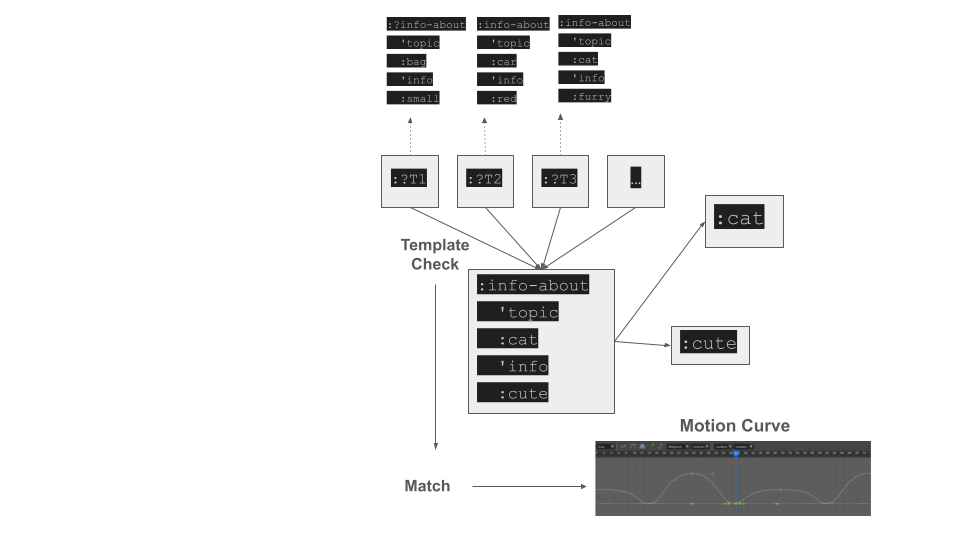
\includegraphics[width = 4in]{chapters/intermediate_blocks/images/top_down_search_template.png}
    \caption{Top-Down Search for Motion Template}
    \label{fig:top_down_search_template}
\end{figure}

The procedurally generated templates can be based on the AZee rule and corresponding motion data. For example, motion curves for the template \texttt{info-about} can be seen in the following figure~\ref{fig:motion_curves_template_procedural}.

\begin{figure}
    \centering 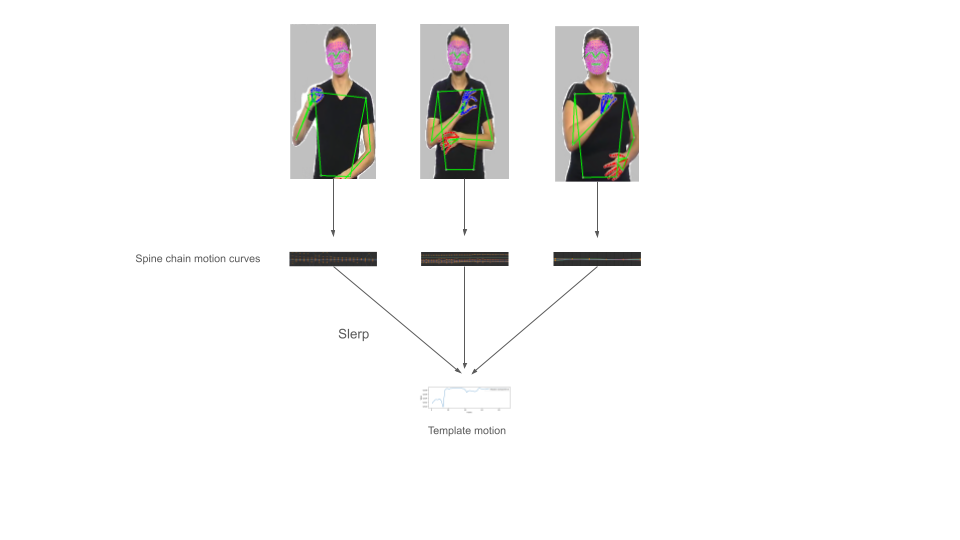
\includegraphics[width = 4in]{chapters/intermediate_blocks/images/motion_curves_template_procedural.png}
    \caption{Procedurally Generated motion curves for template \emph{info-about}}
    \label{fig:motion_curves_template_procedural}
\end{figure}

The template was created by extracting bone rotations as quaternions using mediapipe pose estimation and then converting them into motion curves (figure~\ref{fig:motion_curves_mediapipe}). The final blended rotation can be calculated using Spherical Linear Interpolation (Slerp) between \( n \) quaternions \( q_1, q_2, \dots, q_n \):

\[
q_{\text{blend}} = \text{Slerp}\left(\dots \text{Slerp}\left(\text{Slerp}(q_1, q_2, t_1), q_3, t_2 \right) \dots , q_n, t_{n-1} \right)
\]

Where:
\begin{itemize}
    \item \( t_1, t_2, \dots, t_{n-1} \) are the blend factors for each interpolation step, with \( t_i \in [0, 1] \).
    \item The Slerp between two quaternions \( q_i \) and \( q_j \) is defined as:
    \[
    \text{Slerp}(q_i, q_j, t) = \frac{\sin((1-t)\theta)}{\sin(\theta)} q_i + \frac{\sin(t\theta)}{\sin(\theta)} q_j
    \]
    where \( \theta = \arccos(q_i \cdot q_j) \) is the angle between the quaternions.
\end{itemize}

\begin{figure}
    \centering 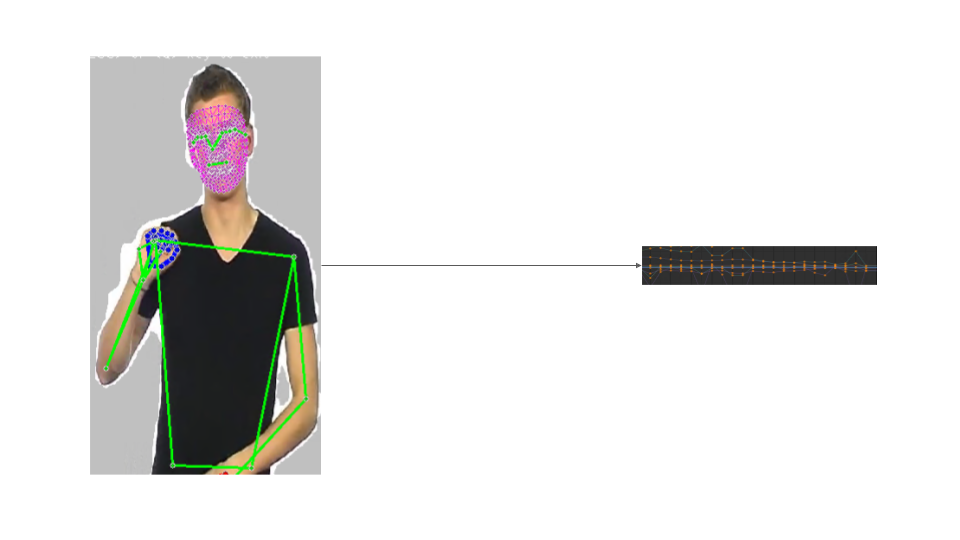
\includegraphics[width = 2.5in]{chapters/intermediate_blocks/images/motion_curves_mediapipe.png}
    \caption{Motion Curves from Mediapipe Pose Estimation}
    \label{fig:motion_curves_mediapipe}
\end{figure}

Figure~\ref{fig:motion_curves_mocap} similar template creation but using AZee annotated motion capture~\cite{bertin2022rosetta}.

\begin{figure}
    \centering 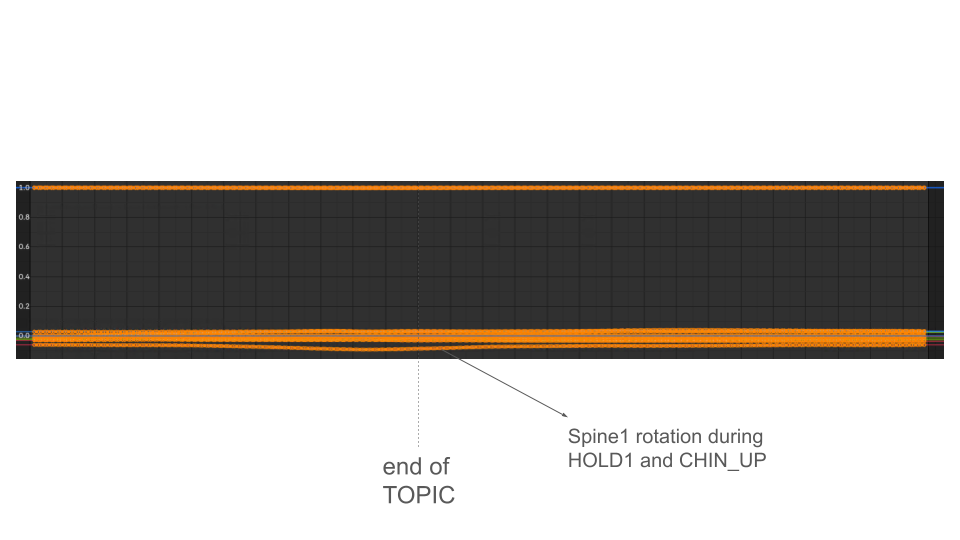
\includegraphics[width = 4in]{chapters/intermediate_blocks/images/motion_curves_mocap.png}
    \caption{Motion Curves from AZee annotated Mocap for the chin up in }
    \label{fig:motion_curves_mocap}
\end{figure}

Lastly, artistically created template for the rule \emph{about-ref} can be seen in the following figure~\ref{fig:motion_curves_template_artist}.

\begin{figure}
     \centering
    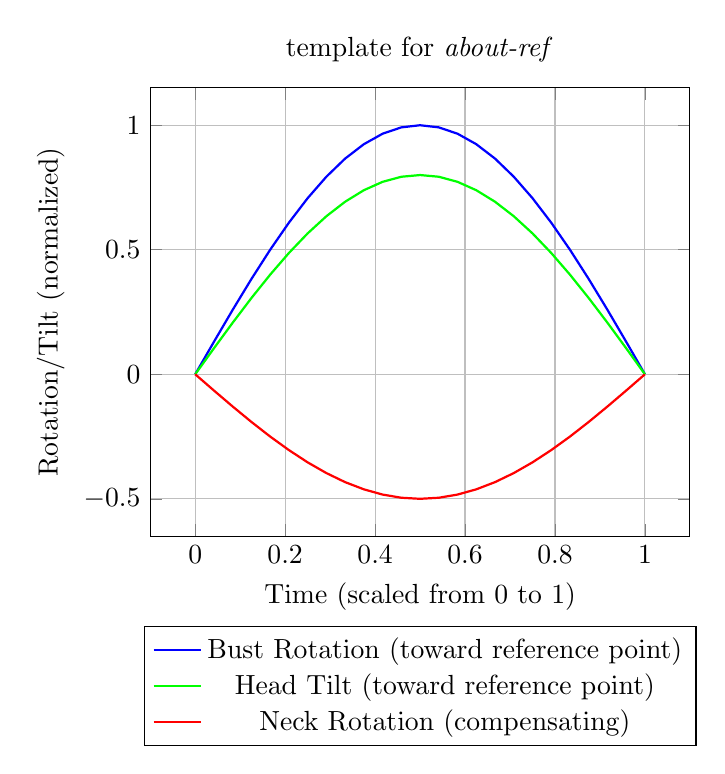
\begin{tikzpicture}
        \begin{axis}[
            title={template for \emph{about-ref}},
            xlabel={Time (scaled from 0 to 1)},
            ylabel={Rotation/Tilt (normalized)},
            grid=major,
            legend style={at={(0.5,-0.2)},anchor=north,legend columns=1} % Legend in two rows
        ]
        % Bust rotation
        \addplot[blue, thick, domain=0:1] {sin(deg(pi*x))};
        \addlegendentry{Bust Rotation (toward reference point)}
        
        % Head tilt
        \addplot[green, thick, domain=0:1] {0.8*sin(deg(pi*x))};
        \addlegendentry{Head Tilt (toward reference point)}
        
        % Neck rotation (compensating)
        \addplot[red, thick, domain=0:1] {-0.5*sin(deg(pi*x))};
        \addlegendentry{Neck Rotation (compensating)}
        
        \end{axis}
    \end{tikzpicture}
    \caption{Artistically Created motion curves for template \emph{about-ref}}
    \label{fig:motion_curves_template_artist}
\end{figure}

\section{Motion Curves}
\label{ch:intermediate_blocks_pose_correction:curves}

Motion curves are a fundamental component of character animation, providing a graphical representation of how a character's movements change over time. By manipulating these curves, animators can control the timing and spacing of movements, ensuring that the animation is realistic and expressive.

\subsection{Skeletal Motion Curves}
\label{ch:intermediate_blocks_pose_correction:curves:skeletal}

The template expression check determines the motion template to be used, which in turn gives us information regarding how a pair of blocks can be connected. However, these motion curves can either effect the skeleton, or the shape keys. For skeleton, these motion curves represent time in x axis, and the joint angle(FK) of the y axis. Each bone has has 4 motion curves (one for each axis of the quaternion rotation).

Figure~\ref{fig:motion_curves_skeletal} shows how motion curves can be used for skeleton for the above example.

\begin{figure}
    \centering 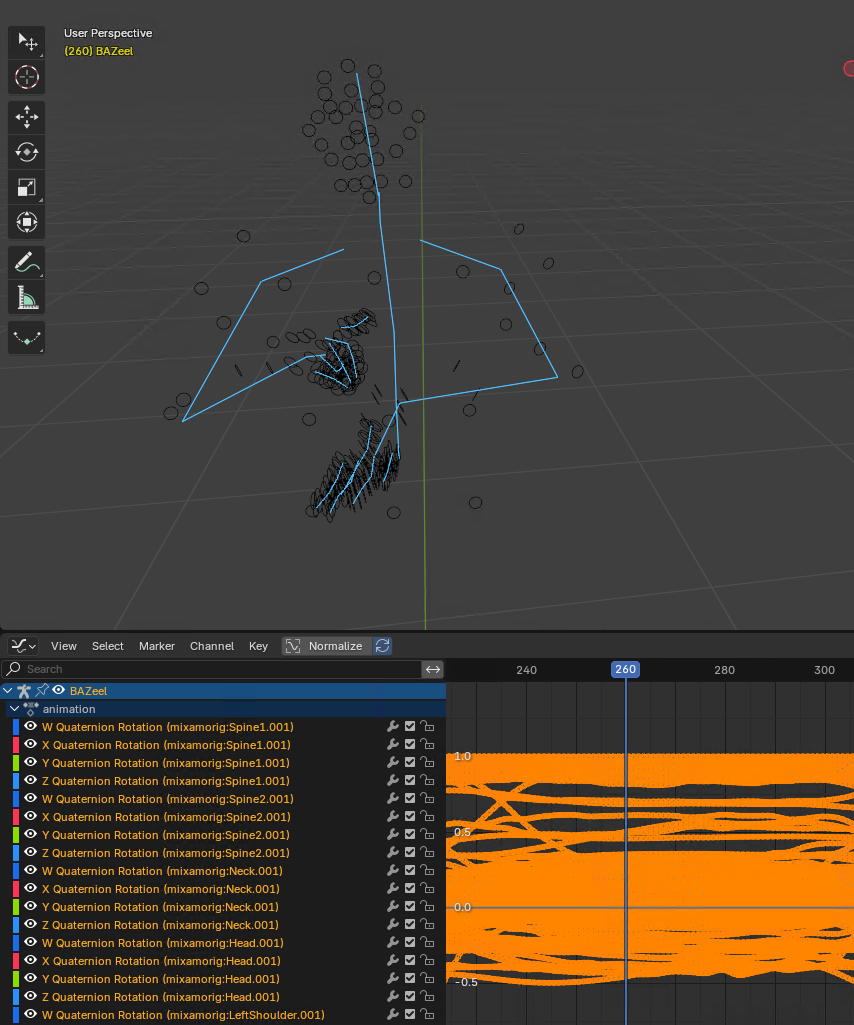
\includegraphics[width = 2.5in]{chapters/intermediate_blocks/images/motion_curves_skeletal.png}
    \caption{Motion Curves for Skeleton}
    \label{fig:motion_curves_skeletal}
\end{figure}

\subsection{Shape Key Motion Curves}
\label{ch:intermediate_blocks_pose_correction:curves:shape_keys}

For shape keys, the motion curves represent time in x axis, and the weight of the shape key in the y axis. Each shape key has one motion curve. Figure~\ref{fig:motion_curves_shape_keys} shows how motion curves can be used for shape keys for the facial expressions of the above example.

\begin{figure}
    \centering 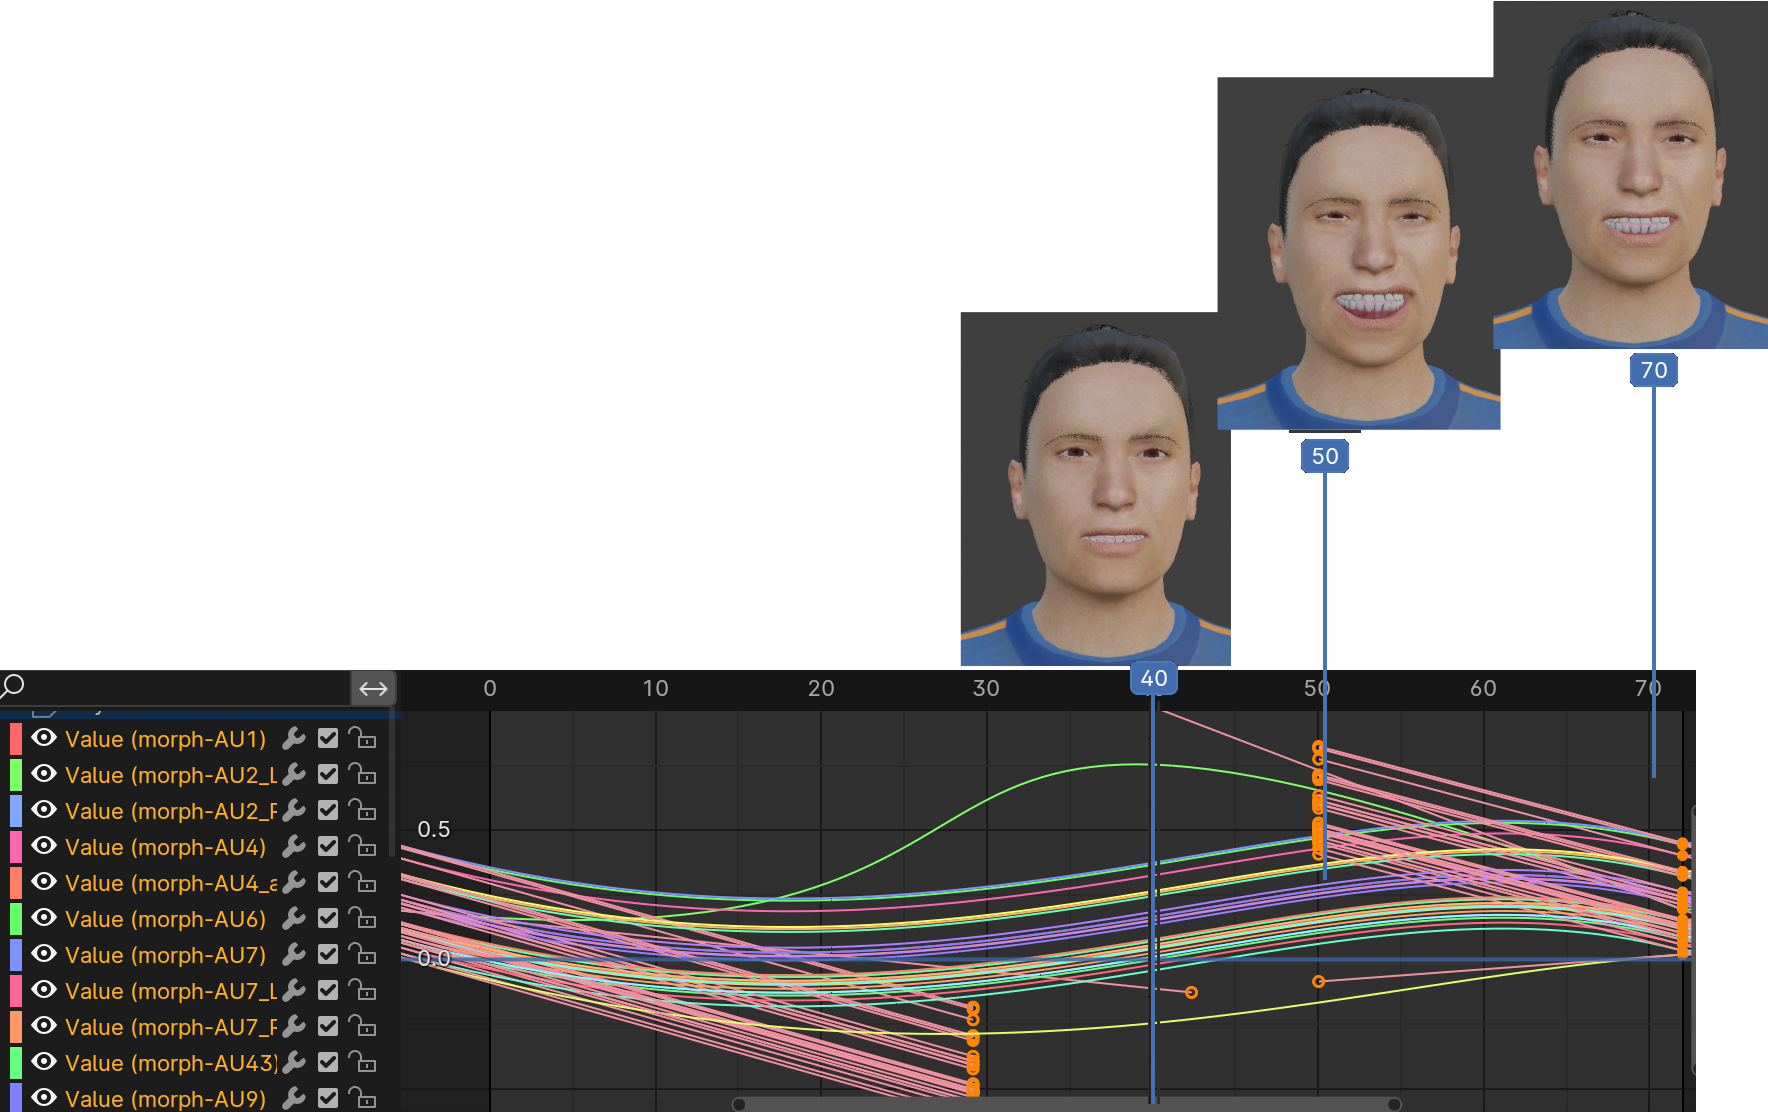
\includegraphics[width = 2.5in]{chapters/intermediate_blocks/images/motion_curves_shape_keys.png}
    \caption{Motion Curves for Shape Keys}
    \label{fig:motion_curves_shape_keys}
\end{figure}

\section{Results}
\label{ch:intermediate_blocks_pose_correction:results}

Table~\ref{tab:intermediate_blocks_comparison}shows the results of the intermediate block generation process. We compare the results of using standard interpolation techniques with the proposed template-based interpolation method. The table shows the difference in naturalness and coherence between the two methods, highlighting the benefits of using motion curves and templates to generate intermediate blocks.

\begin{figure}
    \centering
    \begin{tabular}{|c|c|c|}
    \hline
    \textbf{AZee Rule} & \textbf{Linear Interpolation} & \textbf{Template based Interpolation} \\
    \hline
    TODO & \includegraphics[width=1.5in]{chapters/intermediate_blocks/images/standard_interpolation_todo1.png} & \includegraphics[width=1.5in]{chapters/intermediate_blocks/images/template_interpolation_todo1.png} \\
    \hline
    TODO & \includegraphics[width=1.5in]{chapters/intermediate_blocks/images/standard_interpolation_todo2.png} & \includegraphics[width=1.5in]{chapters/intermediate_blocks/images/template_interpolation_todo2.png} \\
    \hline
    \end{tabular}
    \caption{Comparison with normal interpolation}
    \label{tab:intermediate_blocks_comparison}
\end{figure}

The complete animations can be seen in the following video: \url{todo}

An increase in naturalness when animating using the intermediate blocks technique can be seen. Moreover, this work provides us isnights regarding the motion profile which an AZee rule asbtracts.

todo add this


In the previous chapters, we looked at granularity in sign language animation based on AZee's (linguistic) structure. However, one of the key missing pieces in our study was the ability to shortcut or match a pose on already seen poses. In video games, Motion matching is a technique that dynamically selects the most suitable animation frame or pose from a pre-recorded database based on current input constraints to create fluid, realistic motion. By comparing the motion of the character to a database of motion data, motion matching can generate more realistic and contextually appropriate animations.

The past decade has seen a rise in deep learning technologies in in the field of character animation. These technologies have been used to generate realistic and expressive animations for a wide range of applications, from video games to virtual reality. One of the key challenges in character animation is the generation of natural poses, which requires the ability to capture the nuances of human movement and behavior. 

In this work, we focus on the development of a pose corrector module in our existing synthesis system. We train a pose prior model using a French Sign Language motion capture dataset. The pose prior model captures the typical poses and movements associated with different signs, providing a statistical framework that guides the motion matching process. By learning these priors from a large dataset, our system is able to generate realistic and contextually appropriate sign language poses.

In this chapter, section~\ref{ch:pose_correction:related_work} discusses relevant background work in motion matching and pose correction, focusing on classical methods, data-driven approaches, and the integration of latent space representations. Section~\ref{ch:pose_correction:pose_correction_with_azee} presents the application of thi to the AZee low-level synthesis system, including the preparation of the dataset, training of the Variational Auto Encoder, implementation of pose correction, results and evaluation. Finally, section~\ref{ch:pose_correction:discussion} discusses the implications of integrating pose correction into the AZee system and outlines future directions for research.

\section{Pose Correction with AZee Low Level synthesis}
\label{ch:pose_correction:pose_correction_with_azee}

In this section, we discuss the application of pose correction techniques to the AZee low-level synthesis system. By integrating pose correction, data-driven IK, and latent space representations into the AZee framework, we aim to enhance the realism and expressiveness of sign language animations.

\subsection{Preparing the dataset}
\label{ch:pose_correction:pose_correction_with_azee:dataset}

The first step in integrating pose correction into AZee is to train a Variational Autoencoder (VAE) on set of sign language poses. For this task, we use a dataset of mocap data collected from the Rosetta dataset~\cite{bertin2022rosetta}. The dataset consists of 167066 poses and should capture the diversity of poses and movements associated with different signs, providing a rich source of training data for the VAE.. Since our focus was only on the upper body, we didn't use the facial bones and the lower body for the training. We also retargeted the mocap data to the BAZeel avatar, which is compatible with the AZee skeleton structure (figure~\ref{fig:retargeted}).

\begin{figure}
  \centering 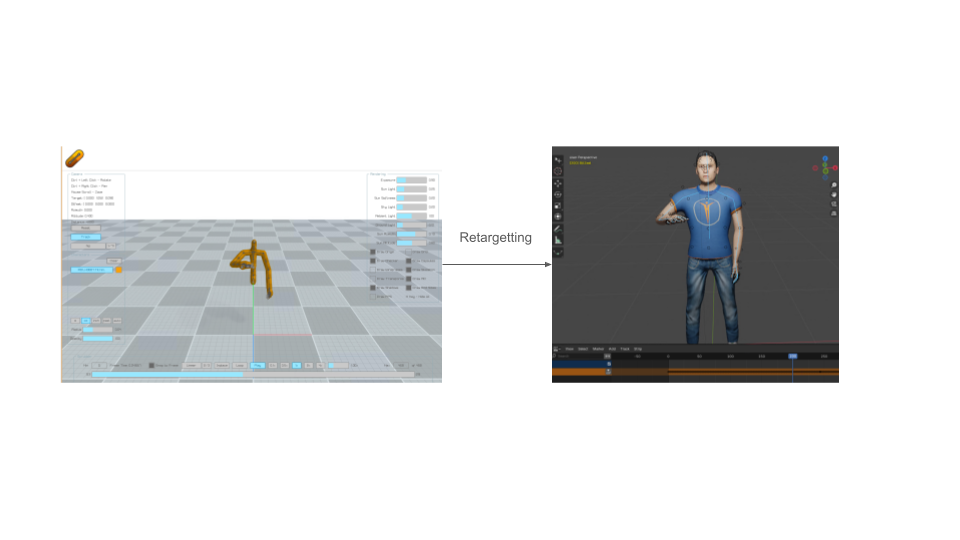
\includegraphics[width = 2.5in]{chapters/pose_correction/images/retargeted.png}
  \caption{Retargeted mocap data to BAZeel avatar}
  \label{fig:retargeted}
\end{figure}

Next, we converted the motion into AZee's FK pose array. The FK pose array consists of the rotation values of each joint in the AZee skeleton (figure~\ref{fig:azee_fk_pose}). This representation is more suitable for the VAE training process, as it captures the pose information in a compact and standardized format.

\begin{figure}
  \centering 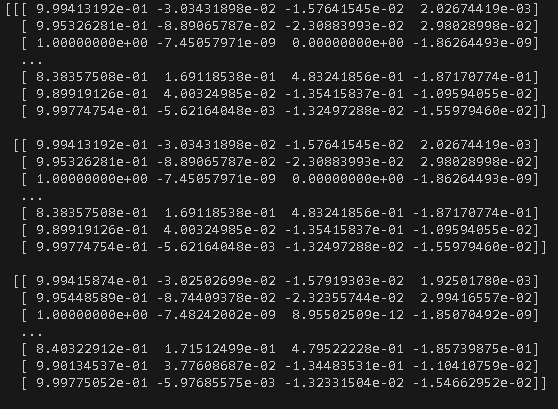
\includegraphics[width = 2.5in]{chapters/pose_correction/images/azee_fk_pose.png}
  \caption{AZee FK Pose Array}
  \label{fig:azee_fk_pose}
\end{figure}

\subsection{Training VPoser}
\label{ch:pose_correction:pose_correction_with_azee:training}

A VAE is a type of generative model that learns a low-dimensional latent space representation of the input data. In the context of character animation, a VAE can be used to capture the distribution of poses in a dataset, allowing for the generation of new poses that are statistically similar to the training data. The VAE consists of an encoder network that maps input poses to a latent space and a decoder network that reconstructs the input poses from the latent space (figure~\ref{fig:vae}).


\begin{figure}[h]
\centering
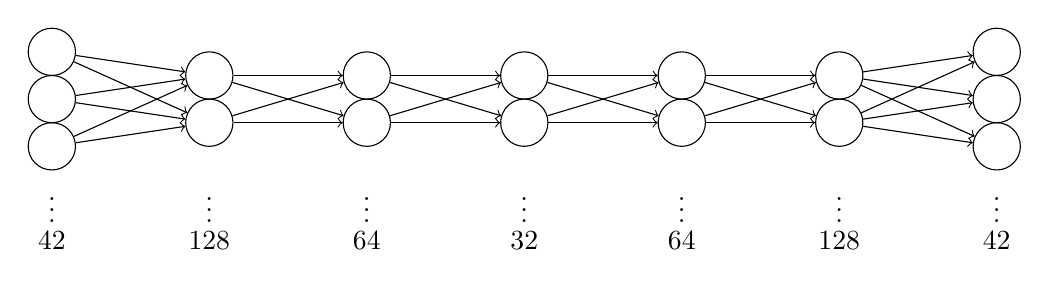
\begin{tikzpicture}[
    every neuron/.style={
        circle,
        draw,
        minimum size=0.6cm
    },
    neuron missing/.style={
        draw=none, 
        scale=1,
        text height=0.333cm,
        execute at begin node=\color{black}$\vdots$
    },
    layer/.style={
        rectangle,
        draw,
        text centered,
        minimum width=2cm
    }
]

% Input Layer
\foreach \i in {1,2,3}
    \node [every neuron/.try, neuron \i/.try] (input-\i) at (0,1.5-\i*0.6) {};

\node at (0,-1) {\vdots};
\node at (0,-1.5) {42};

% Encoder L1
\foreach \i in {1,2}
    \node [every neuron/.try, neuron \i/.try] (L1-\i) at (2,1.2-\i*0.6) {};

\node at (2,-1) {\vdots};
\node at (2,-1.5) {128};

% Encoder L2
\foreach \i in {1,2}
    \node [every neuron/.try, neuron \i/.try] (L2-\i) at (4,1.2-\i*0.6) {};

\node at (4,-1) {\vdots};
\node at (4,-1.5) {64};

% Latent Layer
\foreach \i in {1,2}
    \node [every neuron/.try, neuron \i/.try] (L3-\i) at (6,1.2-\i*0.6) {};

\node at (6,-1) {\vdots};
\node at (6,-1.5) {32};

% Decoder L4
\foreach \i in {1,2}
    \node [every neuron/.try, neuron \i/.try] (L4-\i) at (8,1.2-\i*0.6) {};

\node at (8,-1) {\vdots};
\node at (8,-1.5) {64};

% Decoder L5
\foreach \i in {1,2}
    \node [every neuron/.try, neuron \i/.try] (L5-\i) at (10,1.2-\i*0.6) {};

\node at (10,-1) {\vdots};
\node at (10,-1.5) {128};

% Output Layer
\foreach \i in {1,2,3}
    \node [every neuron/.try, neuron \i/.try] (output-\i) at (12,1.5-\i*0.6) {};

\node at (12,-1) {\vdots};
\node at (12,-1.5) {42};

% Draw the connections
\foreach \i in {1,2,3}
    \foreach \j in {1,2}
        \draw [->] (input-\i) -- (L1-\j);

\foreach \i in {1,2}
    \foreach \j in {1,2}
        \draw [->] (L1-\i) -- (L2-\j);

\foreach \i in {1,2}
    \foreach \j in {1,2}
        \draw [->] (L2-\i) -- (L3-\j);

\foreach \i in {1,2}
    \foreach \j in {1,2}
        \draw [->] (L3-\i) -- (L4-\j);

\foreach \i in {1,2}
    \foreach \j in {1,2}
        \draw [->] (L4-\i) -- (L5-\j);

\foreach \i in {1,2}
    \foreach \j in {1,2,3}
        \draw [->] (L5-\i) -- (output-\j);

\end{tikzpicture}
\caption{Architecture of the VAE}
\label{fig:vae}
\end{figure}

Trained on a dataset containing 167,066 poses. The dataset is divided into training, validation, and test sets, which are loaded using the \texttt{AnimationDS} class from the dataloader. During training, batches of poses are processed, with each batch consisting of 512 samples. The training is carried out on a CUDA-enabled GPU, utilizing mixed precision training for efficiency. The VPoser model architecture consists of a latent space with 32 dimensions (\texttt{latentD}), and the neural network has 512 neurons per layer. 

The loss function used during training includes two primary components: 
\begin{itemize}
    \item \textbf{Reconstruction Loss}: This loss is computed at the joint level by comparing the reconstructed pose with the original pose using L1 loss. An additional pose-level reconstruction loss (L2 loss) is applied during the first 10 epochs to help the model learn better early on.
    \item \textbf{KL Divergence Loss}: The KL divergence regularizes the latent space by enforcing it to follow a standard normal distribution, ensuring that the latent space representation is smooth and continuous.
\end{itemize}

The total loss is the sum of the reconstruction loss and KL divergence loss. The optimization is carried out using the Adam optimizer with a learning rate of $1 \times 10^{-2}$ and weight decay of $0.0001$. A learning rate scheduler is used, which reduces the learning rate by a factor of 0.5 every third of the training epochs. 

\subsection{Implementing Pose Correction}
\label{ch:pose_correction:pose_correction_with_azee:implementation}

With the VAE trained, we can now implement a pose correction system that leverages the learned latent space to match poses generated by the AZee system to the most appropriate pose in the dataset (figure~\ref{fig:pose_correction}).

\begin{figure}
  \centering \includegraphics[width = 2.5in]{chapters/pose_correction/images/pose_correction.png}
  \caption{Pose Correction with VAE}
  \label{fig:pose_correction}
\end{figure}

Algorithm~\ref{alg:pose_correction} outlines the pose correction process. Given a target pose generated by the AZee synthesizor, we first encode the pose into the latent space using the VPoser encoder. We then compute the distance between the encoded pose and each pose in the dataset, selecting the pose with the smallest distance as the best match. Finally, we decode the matched pose back into the AZee FK pose array and apply it to the character.

\begin{algorithm}
  \caption{AZee constraint optimization with pose correction algorithm}
  \label{alg:pose_correction}
  \begin{algorithmic}[1]
  \For{$frame$ \textbf{in} frames}
      \State \texttt{switch\_cursor\_to\_frame($f$)}
      \For{\texttt{parallel\_block \textbf{in} self.parallel\_blocks}}
          \State \texttt{constraints.add(parallel\_block.constraints)}
      \EndFor
      \For{\texttt{constraint \textbf{in} constraints}}
          \State \texttt{constraint.apply($frame$)}
      \EndFor
      \State \texttt{model.pose\_embedding}
      \State \texttt{model.global\_trans}
      \State \texttt{optimizer = \dots}
      \For{\texttt{epoch \textbf{in} range(max\_epochs)}}
          \State \texttt{optimizer.zero\_grad()}
          \State \texttt{\dots}
          \State \texttt{optimizer.step()}
          \If{\texttt{loss.item() < threshold}} \State \texttt{break} \EndIf
      \EndFor
      \State \texttt{posture.keyframe($frame$)}
  \EndFor
  \end{algorithmic}
  \end{algorithm}

\subsection{Results and Evaluation}
\label{ch:pose_correction:pose_correction_with_azee:results}

Snapshots with standard synthesis and synthesis with pose correction and the corresponding AZee code for the same are shown in table~\ref{tab:results}.

\begin{table}
  \centering
  \begin{tabular}{|c|c|c|}
    \hline
    \textbf{Standard Synthesis} & \textbf{Synthesis with Pose Correction} & \textbf{AZee Code} \\
    \hline
    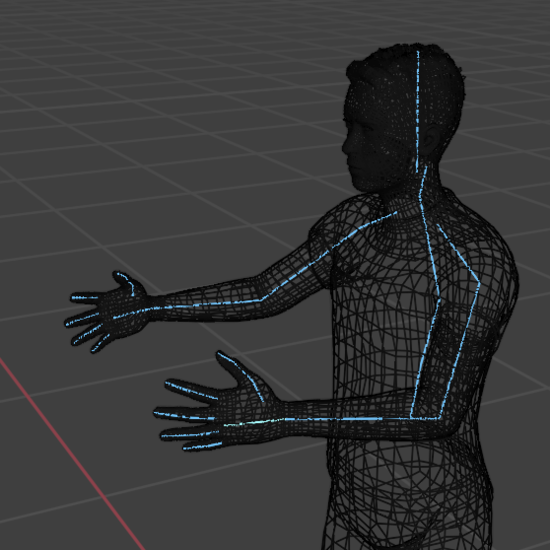
\includegraphics[width = 1.5in]{chapters/pose_correction/images/standard_synthesis_armoire.png} & 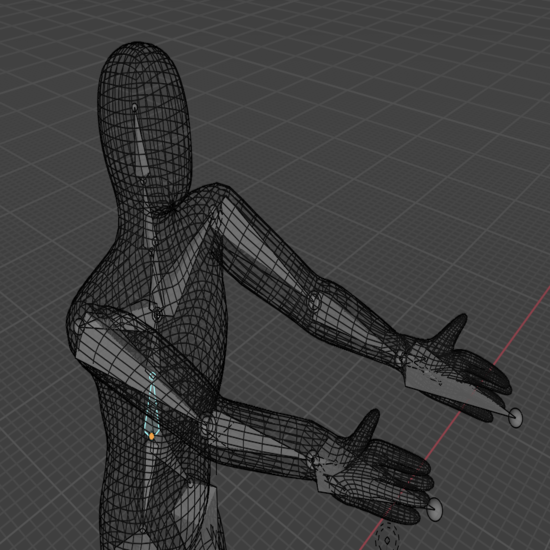
\includegraphics[width = 1.5in]{chapters/pose_correction/images/pose_correction_synthesis_armoire.png} & 
      \emph{:armoire} \\
    \hline
    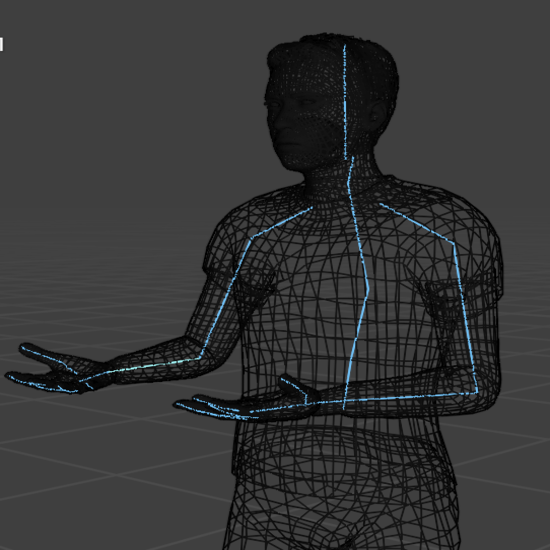
\includegraphics[width = 1.5in]{chapters/pose_correction/images/standard_synthesis_maintenant.png} & 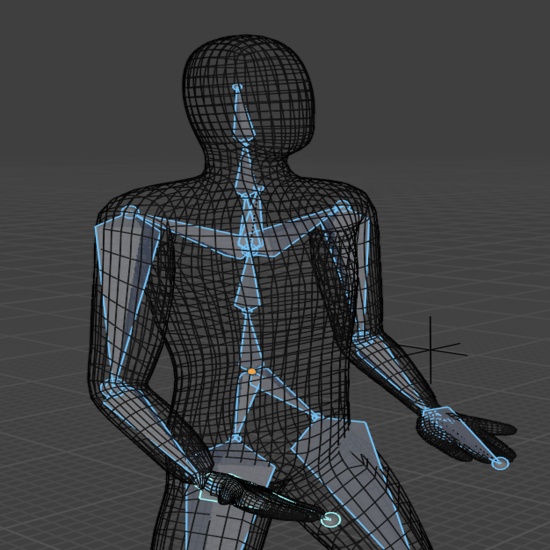
\includegraphics[width = 1.5in]{chapters/pose_correction/images/pose_correction_synthesis_maintenant.png} &
      \emph{:maintenant} \\
    \hline
    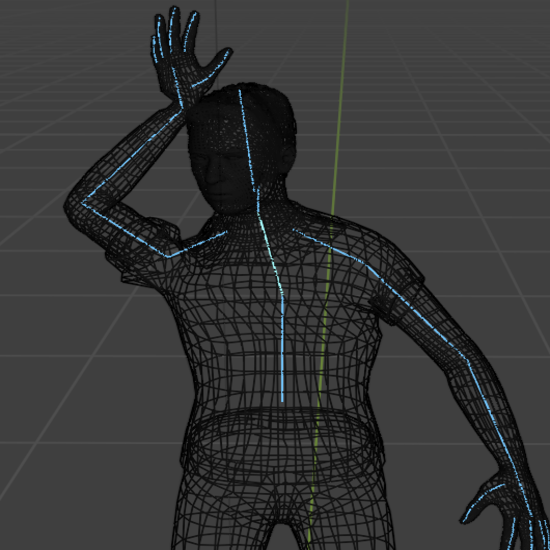
\includegraphics[width = 1.5in]{chapters/pose_correction/images/standard_synthesis_abt_ref_irak.png} & 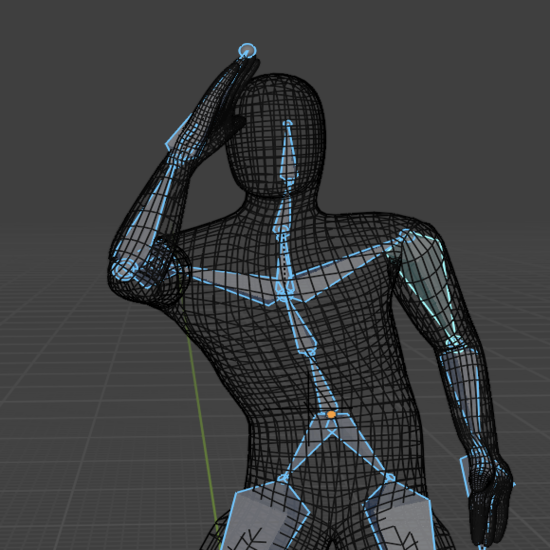
\includegraphics[width = 1.5in]{chapters/pose_correction/images/pose_correction_synthesis_abt_ref_irak.png} &
      \emph{:about-ref(:irak, Rssp)} \\
    \hline
  \end{tabular}
  \caption{Comparison of standard synthesis and synthesis with pose correction}
  \label{tab:results}
\end{table}

The synthesized videos can also be viewed at \href{todo}.

Initial subjective evaluations suggest that the pose correction system produces more natural and contextually appropriate animations compared to standard joint-limit based synthesis. However, due to retargeting losses, the integration of pose correction into Sign Language synthesis is still in the early stages. We also observe that the corrector might change the pose of the character in a way that is not always desirable~\ref{fig:problem_pose_correction}.

\begin{figure}
  \centering 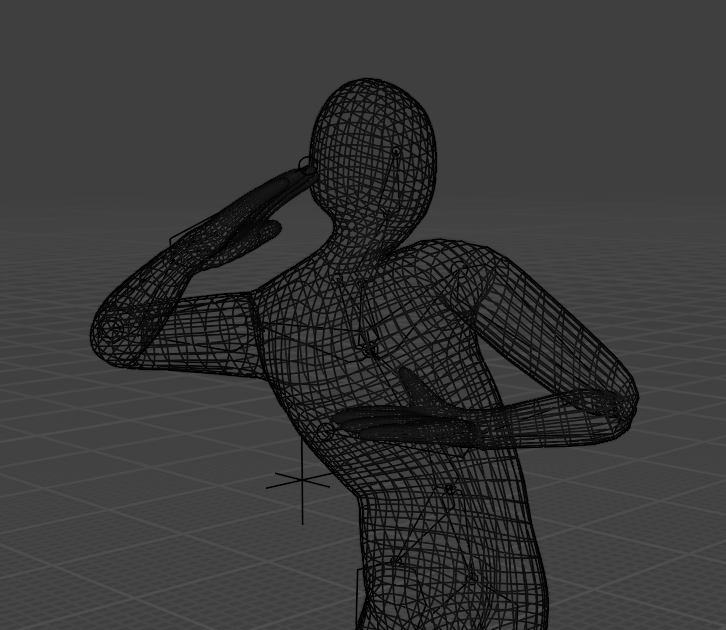
\includegraphics[width = 2.5in]{chapters/pose_correction/images/problem_pose_correction.png}
  \caption{Problems with current correction module}
  \label{fig:problem_pose_correction}
\end{figure}

Lastly, figure~\ref{fig:losses} shows how retargeting the mocap data to the AZee skeleton structure results in a loss of information. This loss can affect the quality of the generated animations and is an area for future improvement.

\begin{figure}
  \centering 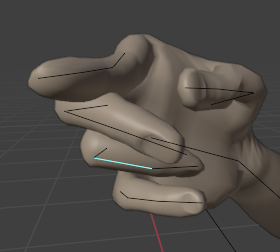
\includegraphics[width = 2.5in]{chapters/pose_correction/images/losses.png}
  \caption{Losses in retargeting mocap data}
  \label{fig:losses}
\end{figure}

\section{Discussion}
\label{ch:pose_correction:discussion}

The integration of pose correction into the AZee system represents a significant advancement in sign language synthesis. By leveraging data-driven IK and latent space representations, we are able to generate more realistic and contextually appropriate sign language animations. This has the potential to enhance the expressiveness and naturalness of sign language avatars, making them more engaging and accessible to users. In some ways, this offfers a new perspective to Sign Language synthesis where the linguistics decides the "what" and the pose corrector decides the "how" of the animation.

For future, posers based on neural distance fields~\cite{tiwari2022pose} or diffusion~\cite{lu2023dposer} could be used for pose correction since the current poser has a bayesian bias. Also, continuity of the trained model with respect to signing spaces could be studied further improving the the learnt pose prior.

While the integration of deep learning into SL synthesis offers numerous advantages, it also introduces new challenges. Data-driven and latent space methods typically require significant computational resources, both during training and inference. This can be a major barrier in real-time applications, where low latency is critical. Also the effectiveness of deep learning models depends heavily on the availability of high-quality training data. In many cases, obtaining sufficient mocap data can be difficult, especially for non-standard or stylized animations. Lastly, while deep learning models can generate realistic and high-quality animations, they often lack the fine-grained control that human animators require. Ensuring that these models produce outputs that align with artistic vision remains a significant challenge.


todo add this

\section{Conclusion and Future Work}
\label{ch:intermediate_blocks_pose_correction:conclusion_and_future_work}

In this chapter, we explored the generation of intermediate blocks in multi-track representations using motion curves and templates. By leveraging the AZee model and motion curves, we were able to create smooth transitions between constrained blocks, enhancing the naturalness and coherence of Sign Language synthesis. The results demonstrate the effectiveness of this approach compared to using standard block interpolation. 

%limitations
While the current system of motion templates proves effective for generating smooth transitions in most body movements, it faces significant challenges when dealing with finer details such as finger articulation. The complexity of finger movements in sign language, especially during rapid transitions, requires high precision in motion curves and templates. Unfortunately, the current implementation lacks the necessary granularity, resulting in robotic transitions. Moreover, capturing thte nuances of coarticulation between handshapes be it with mocap or using pose estimation remains an open challenge.

Another limitation stems from too much data in the motion templates. This might bring in information such as the identity of the signer, which may not always generalize well. This can be mitigated by using a more generalized set of motion templates that can be applied across different signing scenarios.

Future areas to improve this technique could include a more detailed quantitative analysis of motion capture data based on a broader range of AZee rules, as well as further refinement of finger tracking and facial expressions in the motion templates.

Future areas to improve this technique could be a deeper quantitative analysis of mocap data based on more AZee rules. This could help in procedurally creating a more robust set of motion templates that can be used across different signing scenarios.

\end{document}